\documentclass[12pt,a4paper]{report}
\usepackage{graphicx}
\usepackage{hyperref}
\usepackage[all]{hypcap}
\usepackage{times}
\usepackage{xcolor}
\usepackage{tabulary}
\usepackage[top=3cm, bottom=3cm, left=3cm, right=2cm]{geometry}
\hypersetup{
    pdftoolbar=true,        % show Acrobat’s toolbar?
    pdfmenubar=true,        % show Acrobat’s menu?
    pdffitwindow=false,     % window fit to page when opened
    pdfstartview={FitH},    % fits the width of the page to the window
    pdftitle={Report of building a wireless communication system},    % title
    pdfsubject={Report},   % subject of the document
    colorlinks,
    linkcolor=violet,
    citecolor=blue,
    urlcolor=brown
}

\begin{document}
    \title{Report of building a wireless communication system}

    \author{course code: B30SQ \\ by Yifei Jing, Xunyu Kai, Zhi Chai}
    \date{April, 2020}
    \maketitle
    \setlength\parindent{0pt}

\chapter*{Introduction}
The aim of this project is to build a wireless communication system based on what is learn in the course \emph{B30SQ}.
The structure of a communication system is depicted in \hyperref[fig:system_structure]{Figure \ref*{fig:system_structure}}, which composes of a transmitter and a receiver between two computers.
The transmitter composes of a modulator, a frequency converter, an amplifier, and a patch antenna. The receiver includes a patch antenna, an amplifier, a frequency converter, and a demodulator.
In this project, the modulator is implemented using an integrated USB TTL converter, which simply transform the sequence of 0s and 1s from the computer onto electric signal with 0V indicating 0, and 3.3V indicating 1. The frequency converter is achieved using the integrated module.
The amplifiers contain the Low Noise amplifier designed as the first component to the receiver, the op-amps to provide the second level signal amplification at the receiver and the power amplification at the transmitter.
The type of the antenna is the patch antenna, as the principle is easy to be understood. The frequency converter at the receiver end is implemented using a low pass filer.

\begin{figure}[ht]
    \centerline{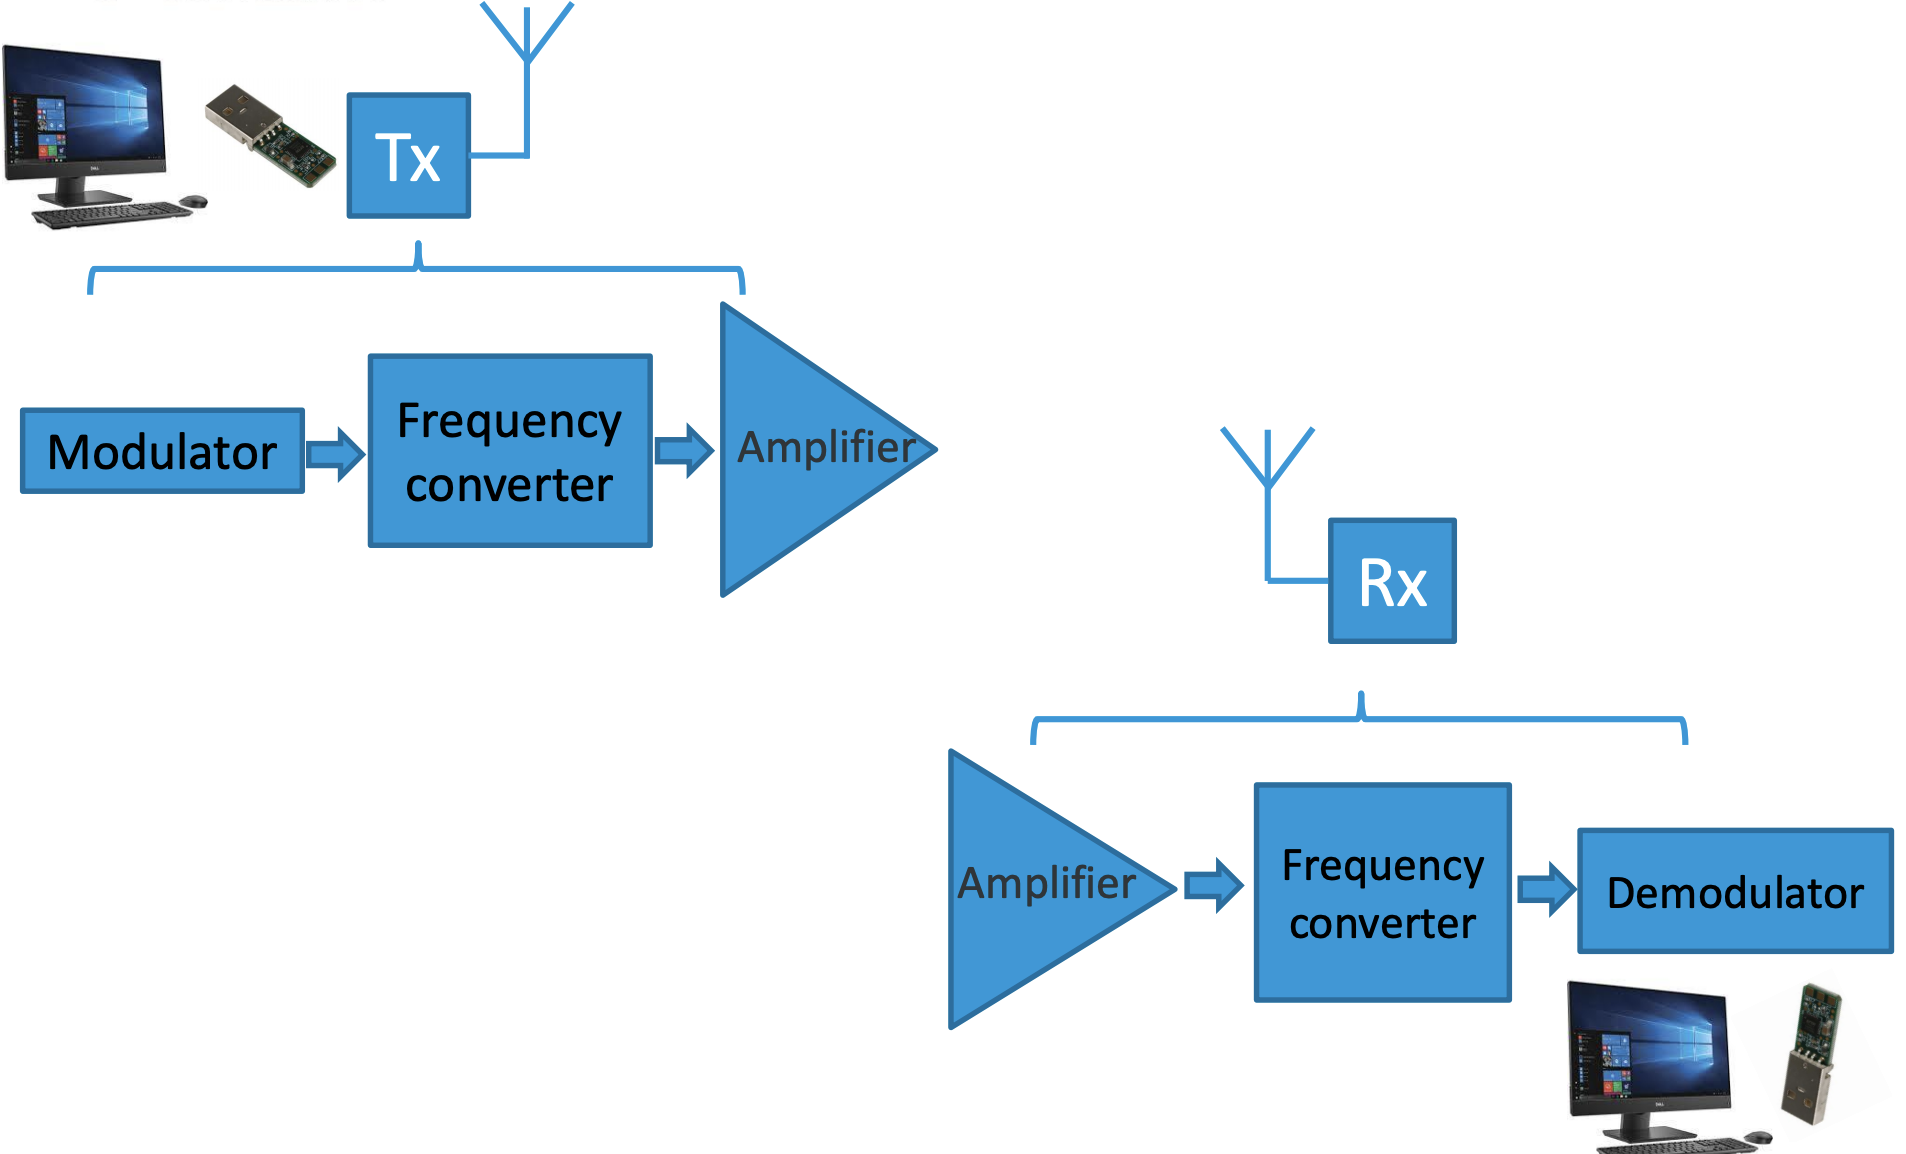
\includegraphics[scale=1]{system_structure}}
    \caption{The structure of a communication system}
    \label{fig:system_structure}
\end{figure}

\section{Operating frequencies}
For the choice of the frequency band, 2400Mhz-2500Mhz is chosen according to ISM: Frequency bands designated for Industrial, Scientific and Medical use.
The reason has been summarized in \hyperref[table:ofea]{Table \ref*{table:ofea}}.

\begin{table}[ht]
    \centering
    \begin{tabulary}{\linewidth}{|L |L| L|}
        \hline
        Frequency band & Standard & Estimation \\ 
        \hline
        433.05 - 434.79 MHz & 5.138 applies. Radiocommunication services must accept harmful interference from ISM. & Antenna size a bit impractical \\
        \hline
        2400 - 2500 MHz & 5.150 applies. Radiocommunication services must accept harmful interference from ISM & Available \\
        \hline
        5725 - 5785 MHz & 5.150 applies. Radiocommunication services must accept harmful interference from ISM. & Elevated cost \\
        \hline
        24.0 - 24.5 GHz & 5.150 applies. Radiocommunication services must accept harmful interference from ISM & Elevated cost and more challenging \\
        \hline
    \end{tabulary}
    \caption{Operating frequencies and estimation of availability}
    \label{table:ofea}
\end{table}

\section{Link budget}
The link budget of a transmitter and a receiver is:
\begin{equation}
    Link \, Budget = L_{FS}(dB) + G_{Tx}(dBi) + G_{Rx}(dBi)
\end{equation}

The term $L_{FS}$ is the free space loss:
\begin{equation}
    L_{FS}(dB) = 32.44 + 20\log{10}{(f(GHz))} + 20\log{10}{(d(meters))}
\end{equation}

Presuming the distance is in the range: $10cm - 2m$, $f = 2.45GHz$, then $L_{FS}$ is in the range $20.2dB - 30.7dB$.
Assuming the gain of the transmitter and the receiver are both $-6dBi$, then the link budget is in the range: $8.2dB - 18.7dB$.
For the requirements that the transmitter and the receiver should be $0dBm$,
\begin{equation}
    P_t(dBm) + G_t(dB) - Link \, Budget + G_r(dB) = P_r(dBm)
\end{equation}
is now re-arranged to: $G_t(dB) + G_r(dB) = Link \, Budget$. Assuming each gain stage is $20dB$, then one stage of amplifier at either transmitter or receiver should be enough.

\chapter*{Patch antenna design}
\chapter*{Amplifier design}
\chapter*{Transmitter's modulator}
\chapter*{Entire system testing}

    
\end{document}